\section{Iteration 10: Decomposition of Other}
\label{add:it10}

\subsection{Step 1: Identify candidate drivers}
\label{add:it10/drivers}

\npar In the first iteration there were quite a lot of requirements delegated to
this component. This requires some selection to take place. This selection is
once again based on the priorities of the quality attributes. However since all
the remaning quality attribute scenarios are (split versions from)
modifiability, they can be easily combined. Furthermore is the remaining
availability quality attribute heavily correlated with M1' concerning the
billing aspect. Therefore the drivers for this iteration are M1', M2, M3' and
Av3.

\npar A short overview of the drivers is given below.

\begin{itemize}
 	\item M1': Dynamic pricing.
  	\begin{itemize}
    	\item The communication between external actors (customer and UIS)
    	and ReMeS concerning billing.
    	\item 
  	\end{itemize}
  	\item M2': Fine-grained metering for enterprises.
  	\begin{itemize}
  	  \item %TODO
  	\end{itemize}
	\item M3': Decentralized electricity generation
  	\begin{itemize}
  	  \item %TODO
  	\end{itemize}
\end{itemize}

\npar M3' is linked with the following use cases:

\begin{itemize}
  \item UC14: Request consumption predictions
  \item UC15: Generate invoide
  \item UC16: Mark invoice paid
\end{itemize}

\npar Because of this relation between M3' and the listed use cases their
functionality will also be adressed. The remaining use cases are delegated to
the other component. %TODO: juist ?

\subsection{Step 2: Choose design concepts}
\label{add:it10/concepts}

\subsubsection{Tactics}
\label{add:it10/tactics}

\paragraph{Modifiability}

\npar For the purpose of modifiability three tactics are selected: anticipate
expected changes, the hiding of information and the use of an intermediary.

\subsubsection{Design Patterns}
\label{add:it10/patterns}

\paragraph{Publisher - Subscriber}

\npar The \emph{Publisher - Subscriber} pattern is in this context particularly useful due to
the inherently unknown parties potentially interested in certain messages. E.g. When
later in time dynamic pricing is introduced it is simply possible for the other
interested parties (customers, HAS, etc.) to subscribe to these events. So this
pattern aids in realizing the anticipate expected changes tactic.

\paragraph{Facade}

\npar To shield the system and it's external actors (i.e. The third party
billing service and utility providers) the \emph{Facade} pattern is interesting.
The pattern suggests a single point of access for both of the aforementioned
actors to access but there is a possibility of bypassing this accesspoint in a
number of sophisticated scenarios. In the context of this decomposition a slight
variation of this pattern is used, this will be explained below. The shielding
functionality of the facade reflects the use of an intermediary (and in a sense
the hiding of information). Notice that there is no explicit design pattern used
for the hiding of information but this is mainly realized in the use of
interfaces for all different components.

\subsection{Step 3: Instantiate architectural elements and allocate responsibilities}
\label{add:it10/elements}

\begin{figure}[H]
	\begin{centering}
		% TODO Figure
		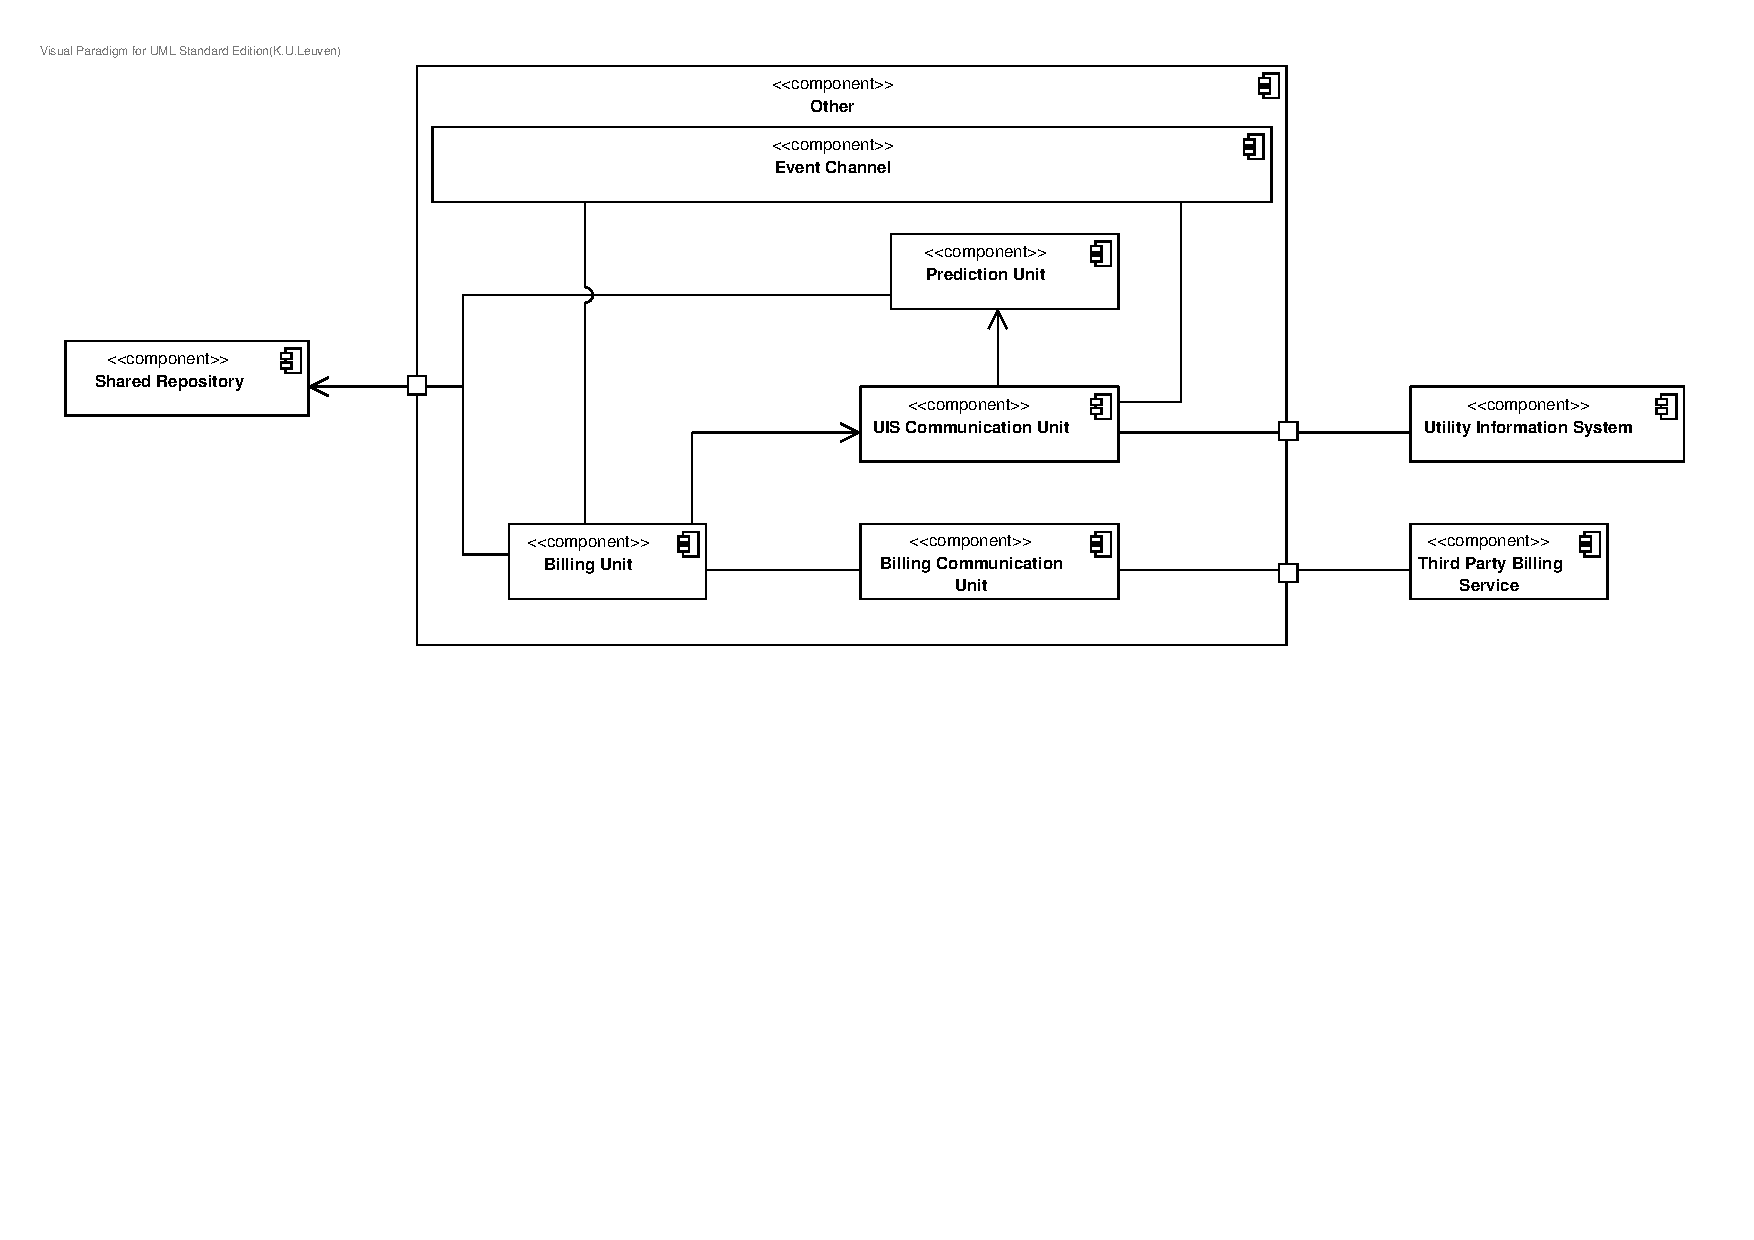
\includegraphics[width=\textwidth]{figs/add-it10-elements.pdf}
		\caption{Overview of the instantiated child elements in the other component}
		\label{fig:add/it10/decomposition}
	\end{centering}
\end{figure}

\npar The full decomposition of this iteration can be viewed in figure
\ref{fig:add/it10/decomposition}. In the subsection below each of the components
will be discussed. 

\subsubsection{Price Channel}

\npar This component is the instantiation of the \emph{Publisher - Subscriber}
pattern's ``Change Propagation Infrastructure''. Its responsibilities are the
handling of subscriptions and publications to certain events. Users of this
channel can be invoke one of the methods of it's interface,
\interface{BillingChannel}. These are discussed in \ref{add:it8/interfaces}.

\subsubsection{Prediction Unit}

\npar The prediction unit is responsible for fetching the consumption
histories of all customers, processing (i.e. running all sorts of
prediction algorithms on the fetched data)and exporting. Therefore it offers a
\interface{Prediction} interface.

\subsubsection{Billing Unit}

\npar The responsibility of this unit is limited to the generation of invoices.
Ths includes determining that an invoice should be constructed, fetching all the
relevant consumption data and constructing the invoice. The constructed invoice
is then sent towards the billing communication unit through the
\interface{BillingReceive} interface. One more task is assigned to this
component, namely the marking of paid invoices. To retrieve all data the billing
unit needs, first of all it has to have access through the internal ReMeS
customer database (through the \interface{CustomerProfile} interface).
Secondly, it needs to be able to contact the UIS. This is done through the
\interface{CustomerInformation}.

\subsubsection{UIS Communication Unit}

\npar This unit is the first of two units responsible for communication with
external actors in respect to billing and prediction. In section
\ref{add:it8/patterns} we discussed the usage of a slight variant of the
\emph{Facade} pattern. The deviation of the standard pattern lies firstly in the
usage of two communication units instead of one single point of access.
Secondoly there is no bypassing of this communication (not even in a limited
number of scenarios).

\npar This component interacts with three other components. The first one,
Utility information system, is used for all information needed by ReMeS that is
stored by the utility company. The second one, prediction unit, is used to
acquire prediction statistics for a certain utility company. Besides using
interfaces the UIS communication unit off course offers interfaces itself. It
offers two main services towards other components: one towards the billing unit
and one towards the UIS. The former service includes the retrieval of customer
data that is kept by the UIS. The latter one is more of a consultation service
where the UIS can request predictions.

\subsubsection{Billing Communication Unit}

\npar The responsibility of this unit is the handling of all information between
ReMeS and external actors regarding billing. It has two major duties. The first
is to allow invoices to be sent towards the third party billing service after
the invoice has been constructed off course. The second task is to provide a
possibility for all notification that need to be sent towards ReMeS concerning
the payment of invoices.

\npar The billing communication unit also uses functionality which is reflected
in the usage of the billing unit and third party billing service. The former one
is used to sent the notification of a payment towards the billing unit. It uses
the third party billing service in the sense of sending it the right documents.

\subsection{Step 4: Define interfaces for instantiated elements}
\label{add:it10/interfaces}

\subsubsection{Event Channel}

\paragraph{PriceChannel}
% TODO parameter van subscribe = juist?
\npar This is a quite simple interface and offers only two methods. The first
method is a \method{publish{PriceEvent}} method which can be invoked by
Publishers (in this context \method{publish} will be called by UIS communication
unit to make price updates available to all interested parties). Callers the
second method, \method{subscribe(PriceFilter)}, will receive events which
match the specified filter.

\subsubsection{Prediction Unit}

\paragraph{PredictionAPI}

\npar Only one method is included in the \interface{PredictionAPI} interface,
namely \method{getConsumptionPredictions(UtilityProvider)}. This method will
fetch all the relevant data (i.e. the data from all the customers of the given
utility provider). The next step is to run several (machine learning-based)
prediction algorithms for analysis. When this is result is computed it is
returned towards the invoker of the method.

\subsubsection{Billing Unit}

\paragraph{BillingReceive}

\npar This interface has only one method, namely \method{markPaid(String)}. It
serves to notify the billing unit when an invoice is paid so it can be stored in
the ReMeS database.

\subsubsection{Billing Communication Unit}

\paragraph{BillingSend}

\npar This interface has once again only one method, \method{send(Invoice)}.
This method is to be invoked by the billing unit once it has constructed an
invoice that needs to be sent to the third party billing service.

\paragraph{BillingCommunication}

\npar This interface has only one method, namely \method{markPaid(String)}. It
serves to notify the billing unit when an invoice is paid so it can be stored in
the ReMeS database.

\subsubsection{UIS Commmunication Unit}

\paragraph{CustomerInformation}

\npar The \interface{CustomerInformation} interface offers two methods:
\method{getContractInformation(Customer)} and
\method{getPricingInformation(Date)}. The former encloses the collection of all
kind of information which is useful when drafting an invoice for a given
customer. The latter encompasses information concerning the price (e.g.
night rate discounts, etc.).

\paragraph{UISCommunication}
%zelfde probleem als bij billingCOmmunication, deze interface is praktisch
% dezelfde als die van Prediction (de communiation blokken zijn uiteindelijk
% maar facades.)
\npar This interface offers one method, namely
\method{getConsumptionPrediction(UtilityProvider)}. A call to this
method will dispatched to the \interface{PredictionAPI} interface.

\begin{figure}[H]
	\begin{centering}
		% TODO Figure 
		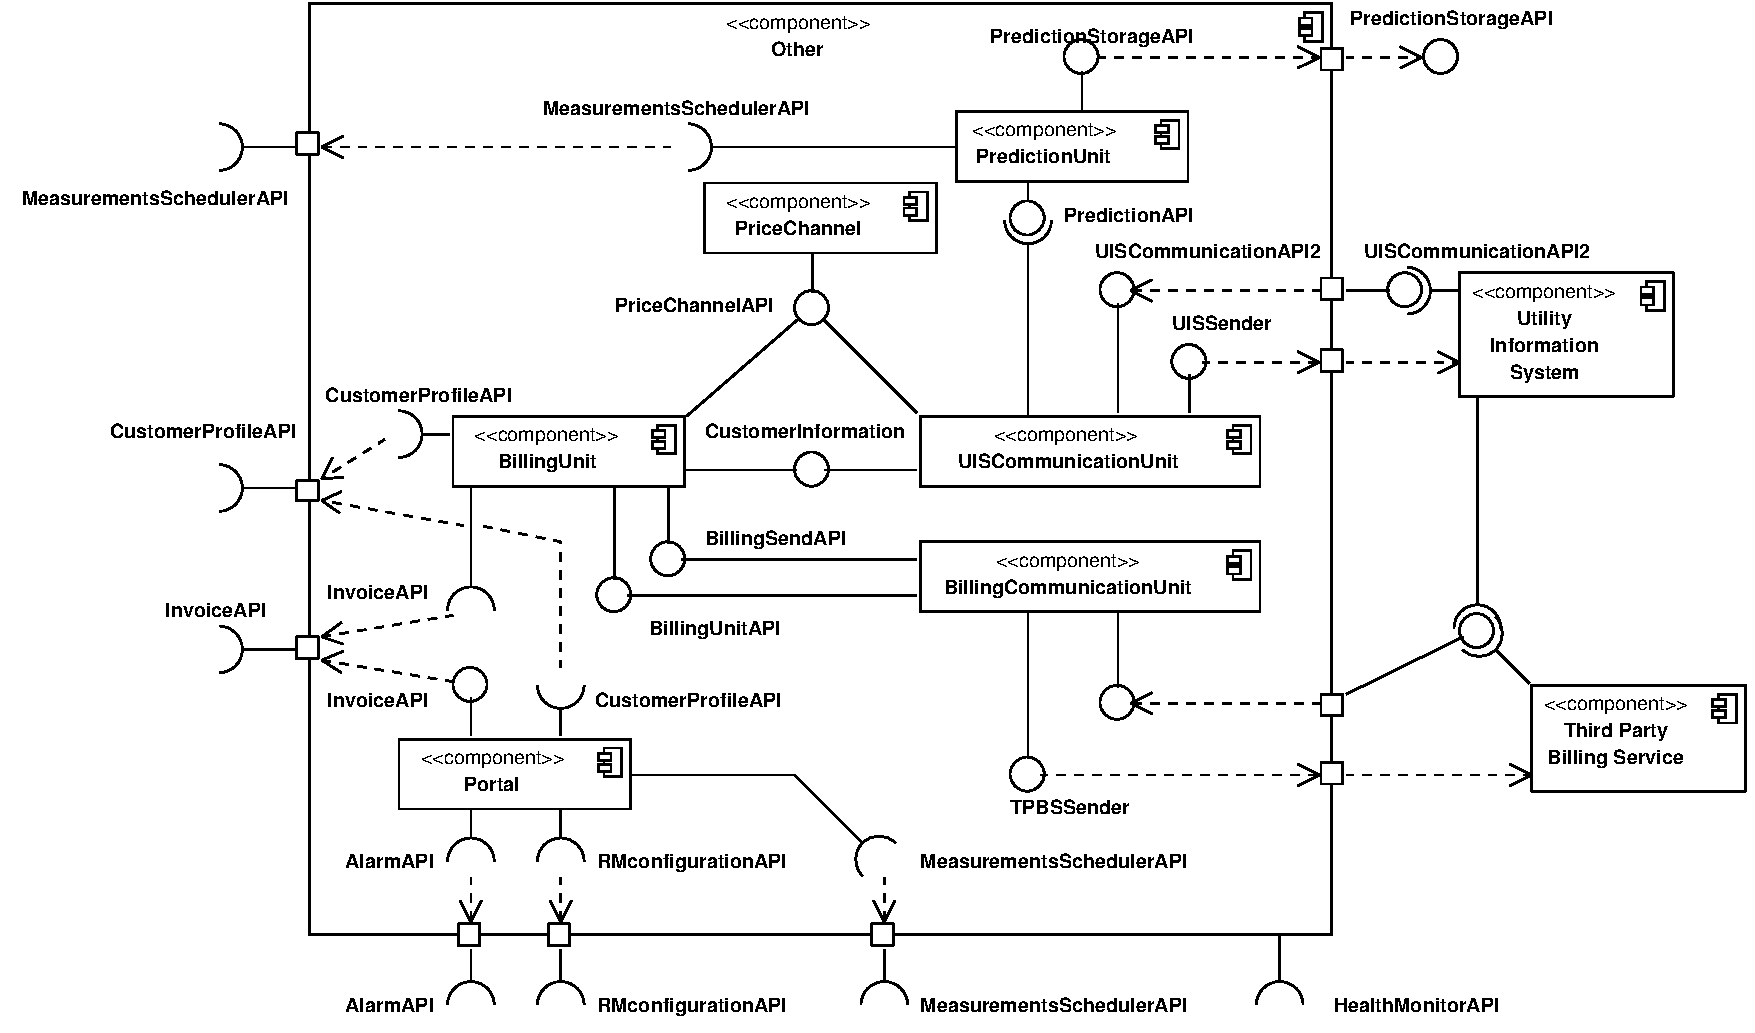
\includegraphics[width=\textwidth]{figs/add-it10-interfaces.pdf}
		\caption{Overview of the interfaces and components in the Other Component}
		\label{fig:it10/interfaces}
	\end{centering}
\end{figure}

\subsection{Step 5: Verify and refine}
\label{add:it10/verification}

\npar All quality attribute drivers and assigned use cases were resolved in
this iteration. There are still, however, a number of non resolved use cases and
one quality attribte which are listed below. The quality attribute is
delegated to the billing communication unit. The use cases are all delegated to
the Other component.

%TODO: correct (dat van de use cases) ?

\begin{itemize}
  \item Billing Communication Unit:
  \begin{itemize}
    \item Av3 : Third Party Billing Service Failure
  \end{itemize}
  \item Other
  \begin{itemize}
  	\item UC1 : Log in
  	\item UC2 : Log off
  	\item UC3 : Register customer
  	\item UC4 : Unregister customer
  	\item UC5 : Associate device to customer
  	\item UC6 : Customize customer profile
 	\item UC11: Operate actuator remotely
  	\item UC12: Set alarm recipients
  \end{itemize}
\end{itemize}
